\documentclass{article}\usepackage{graphicx, color}
%% maxwidth is the original width if it is less than linewidth
%% otherwise use linewidth (to make sure the graphics do not exceed the margin)
\makeatletter
\def\maxwidth{ %
  \ifdim\Gin@nat@width>\linewidth
    \linewidth
  \else
    \Gin@nat@width
  \fi
}
\makeatother

\definecolor{fgcolor}{rgb}{0.2, 0.2, 0.2}
\newcommand{\hlnumber}[1]{\textcolor[rgb]{0,0,0}{#1}}%
\newcommand{\hlfunctioncall}[1]{\textcolor[rgb]{0.501960784313725,0,0.329411764705882}{\textbf{#1}}}%
\newcommand{\hlstring}[1]{\textcolor[rgb]{0.6,0.6,1}{#1}}%
\newcommand{\hlkeyword}[1]{\textcolor[rgb]{0,0,0}{\textbf{#1}}}%
\newcommand{\hlargument}[1]{\textcolor[rgb]{0.690196078431373,0.250980392156863,0.0196078431372549}{#1}}%
\newcommand{\hlcomment}[1]{\textcolor[rgb]{0.180392156862745,0.6,0.341176470588235}{#1}}%
\newcommand{\hlroxygencomment}[1]{\textcolor[rgb]{0.43921568627451,0.47843137254902,0.701960784313725}{#1}}%
\newcommand{\hlformalargs}[1]{\textcolor[rgb]{0.690196078431373,0.250980392156863,0.0196078431372549}{#1}}%
\newcommand{\hleqformalargs}[1]{\textcolor[rgb]{0.690196078431373,0.250980392156863,0.0196078431372549}{#1}}%
\newcommand{\hlassignement}[1]{\textcolor[rgb]{0,0,0}{\textbf{#1}}}%
\newcommand{\hlpackage}[1]{\textcolor[rgb]{0.588235294117647,0.709803921568627,0.145098039215686}{#1}}%
\newcommand{\hlslot}[1]{\textit{#1}}%
\newcommand{\hlsymbol}[1]{\textcolor[rgb]{0,0,0}{#1}}%
\newcommand{\hlprompt}[1]{\textcolor[rgb]{0.2,0.2,0.2}{#1}}%

\usepackage{framed}
\makeatletter
\newenvironment{kframe}{%
 \def\at@end@of@kframe{}%
 \ifinner\ifhmode%
  \def\at@end@of@kframe{\end{minipage}}%
  \begin{minipage}{\columnwidth}%
 \fi\fi%
 \def\FrameCommand##1{\hskip\@totalleftmargin \hskip-\fboxsep
 \colorbox{shadecolor}{##1}\hskip-\fboxsep
     % There is no \\@totalrightmargin, so:
     \hskip-\linewidth \hskip-\@totalleftmargin \hskip\columnwidth}%
 \MakeFramed {\advance\hsize-\width
   \@totalleftmargin\z@ \linewidth\hsize
   \@setminipage}}%
 {\par\unskip\endMakeFramed%
 \at@end@of@kframe}
\makeatother

\definecolor{shadecolor}{rgb}{.97, .97, .97}
\definecolor{messagecolor}{rgb}{0, 0, 0}
\definecolor{warningcolor}{rgb}{1, 0, 1}
\definecolor{errorcolor}{rgb}{1, 0, 0}
\newenvironment{knitrout}{}{} % an empty environment to be redefined in TeX

\usepackage{alltt}
\usepackage{pdflscape}
\usepackage{caption}
\usepackage{rotating}
\usepackage{graphicx}
\IfFileExists{upquote.sty}{\usepackage{upquote}}{}
\begin{document}

\title{Williamstown Weather Package}
\author{Angel Zhou and Michaela Kane}
\maketitle

\begin{figure}
\section*{Introduction}

The Williamstown Weather package takes data tables of the temperatures
(in degrees Farenheit) of Williamstown, MA and, from the tables,
extracts the desired data sets of date and temperature and puts them
into a new data frame.

\section*{The Read Weather 1 Function}
The \verb+readWeather1+ function takes data formatted in a similar
manner to that of the table at
\verb+http://web.williams.edu/weather/100_history.php?type=Temperature+,
and creates a data frame directly comparing the date to the monthly
temperatures in Williamstown, MA from 1892 to 2010. This function
accepts as parameters the \verb+fileName+ (the name of the text file
of data to be used), the logical \verb+h+ value (if \verb+TRUE+, it
keeps the current header), and the \verb+dateFormat+ (what format the
date object should be read in as).

\begin{knitrout}
\definecolor{shadecolor}{rgb}{0.969, 0.969, 0.969}\color{fgcolor}\begin{kframe}
\begin{alltt}
\hlfunctioncall{library}(lubridate)
\hlfunctioncall{library}(reshape)
\end{alltt}


{\ttfamily\noindent\itshape\color{messagecolor}{\#\# Loading required package: plyr}}

{\ttfamily\noindent\itshape\color{messagecolor}{\#\# \\\#\# Attaching package: 'plyr'}}

{\ttfamily\noindent\itshape\color{messagecolor}{\#\# The following object is masked from 'package:lubridate':\\\#\# \\\#\#\ \ \ \  here}}

{\ttfamily\noindent\itshape\color{messagecolor}{\#\# \\\#\# Attaching package: 'reshape'}}

{\ttfamily\noindent\itshape\color{messagecolor}{\#\# The following object is masked from 'package:plyr':\\\#\# \\\#\#\ \ \ \  rename, round\_any}}

{\ttfamily\noindent\itshape\color{messagecolor}{\#\# The following object is masked from 'package:lubridate':\\\#\# \\\#\#\ \ \ \  stamp}}\begin{alltt}
\hlfunctioncall{library}(ggplot2)
x <- \hlfunctioncall{read.table}(\hlstring{"monthlyTemp.txt"}, header = TRUE)
y <- \hlfunctioncall{melt}(x, id = \hlstring{"Year"})
stringDates <- \hlfunctioncall{paste}(y$variable, y$Year, 20, sep = \hlstring{"/"})
Date <- \hlfunctioncall{as.Date}(stringDates, format = \hlstring{"%b/%Y/%d"})
y$Temperatures <- y$value
months <- \hlfunctioncall{months}(Date, abbr = TRUE)
months_fac = \hlfunctioncall{factor}(months, levels = month.abb)
y$Month <- \hlfunctioncall{sort}(months_fac)
p <- \hlfunctioncall{ggplot}(y, \hlfunctioncall{aes}(Date, Temperatures))
p <- p + \hlfunctioncall{geom_point}(size = 1)
p <- p + \hlfunctioncall{geom_line}(size = 0.2)
p <- p + \hlfunctioncall{xlab}(\hlstring{"Year"})
\end{alltt}
\end{kframe}
\end{knitrout}

\end{figure}

\begin{landscape}
  \begin{figure}
\begin{knitrout}
\definecolor{shadecolor}{rgb}{0.969, 0.969, 0.969}\color{fgcolor}
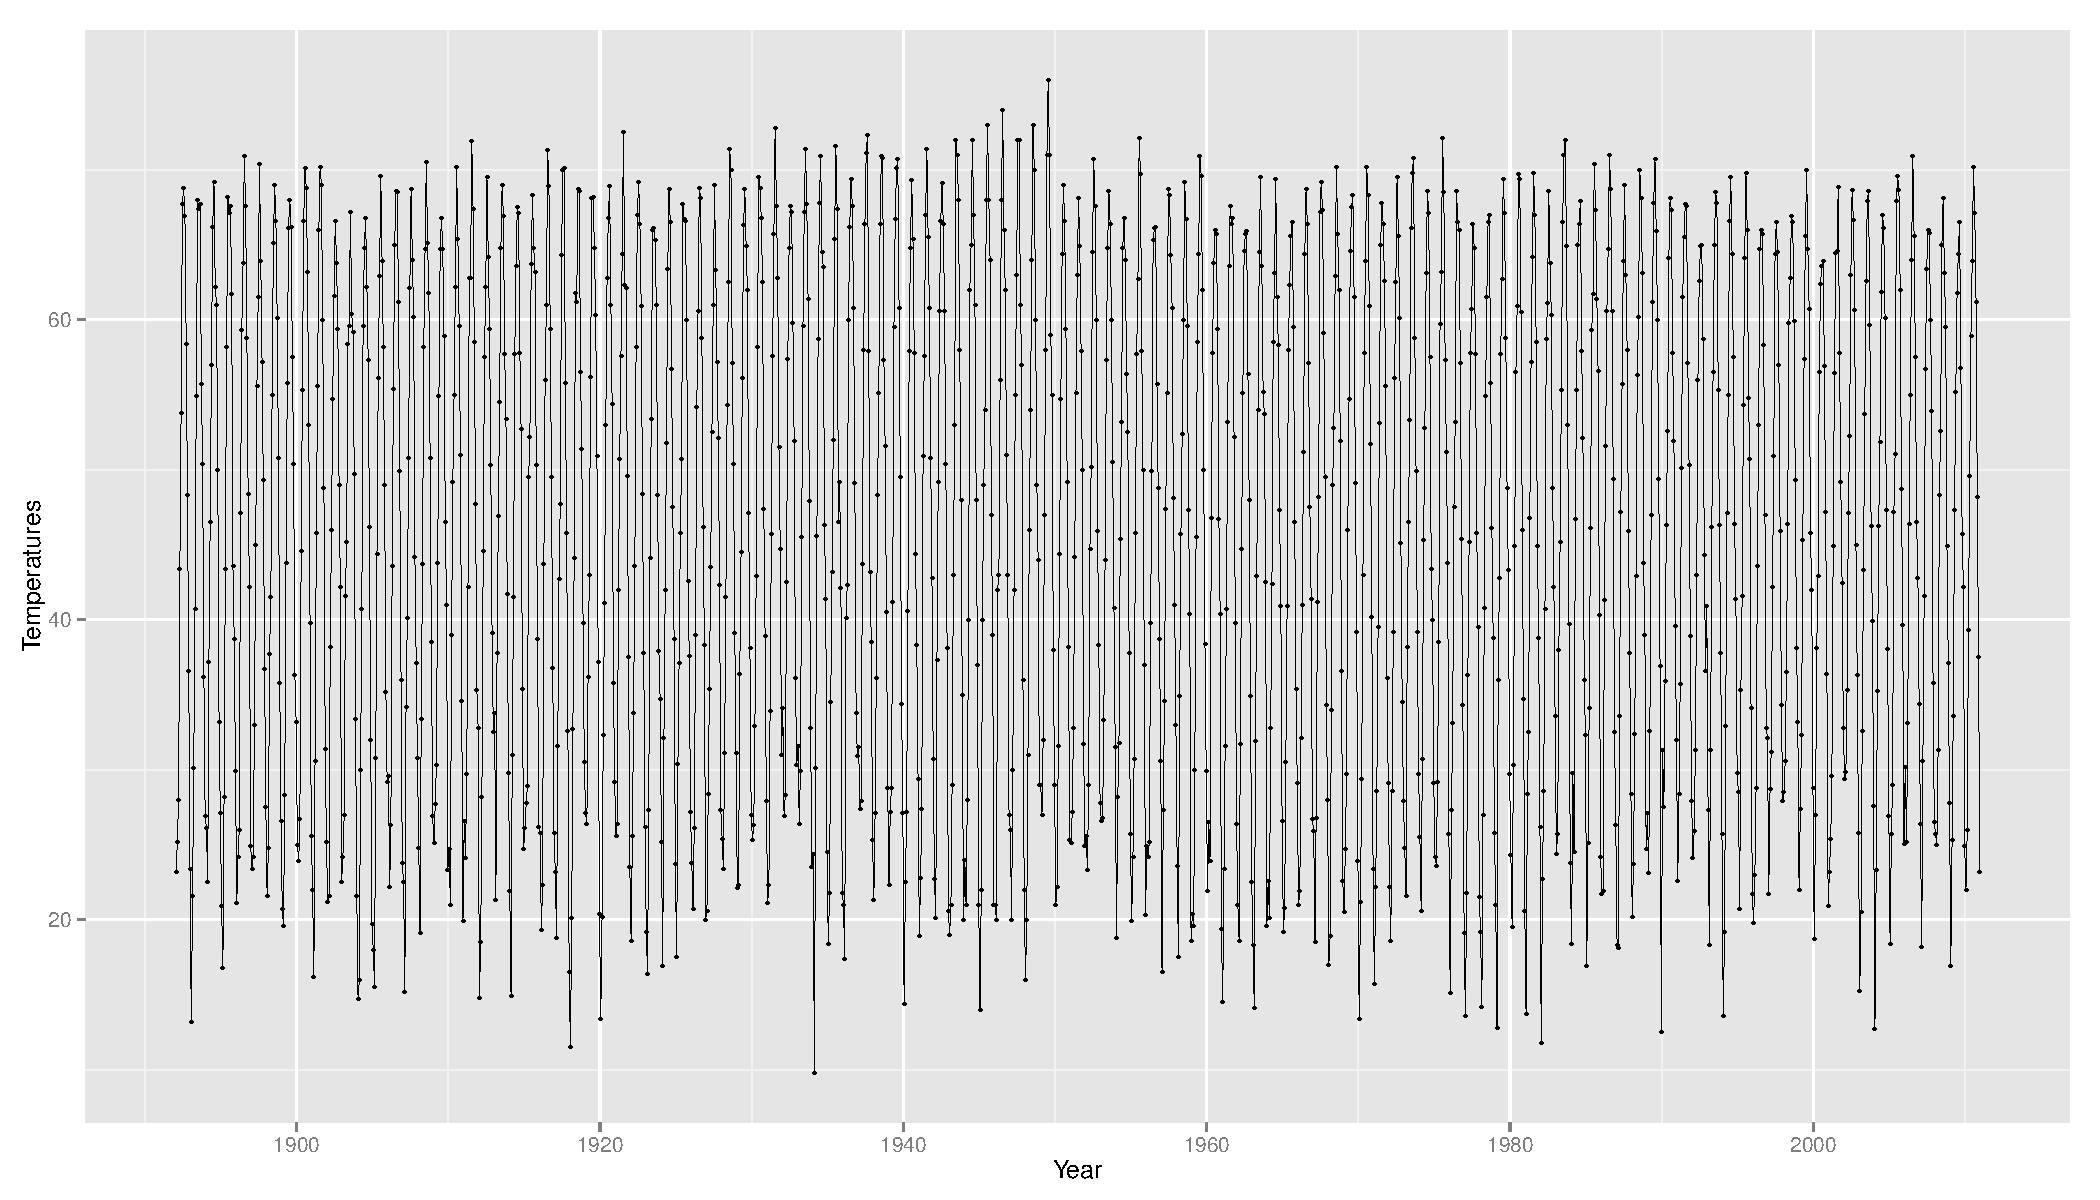
\includegraphics[width=\maxwidth]{figure/graph1Landscape} 

\end{knitrout}

\caption{This scatterplot illustrates the monthly temperatures in degrees
  Farenheit of Williamstown, Massachusetts as recorded from January
  1892 to December 2010.}
\end{figure}
\end{landscape}

\subsection{Analysis}
Because the data was collected monthly over a term of over 200 years, the plot is quite crowded. However, we notice
that the fluctuation in temperature over the course of each year has not changed significantly despite theories regarding
global warming and climate change. This could be due to Williamstown's relatively remote location or to its low population,
but overall very little change is seen between the relative maximums/minimums in temperature.

\begin{figure}
\begin{knitrout}
\definecolor{shadecolor}{rgb}{0.969, 0.969, 0.969}\color{fgcolor}\begin{kframe}
\begin{alltt}
bp <- \hlfunctioncall{ggplot}(y, \hlfunctioncall{aes}(Month, Temperatures)) + \hlfunctioncall{geom_boxplot}()
bp
\end{alltt}
\end{kframe}
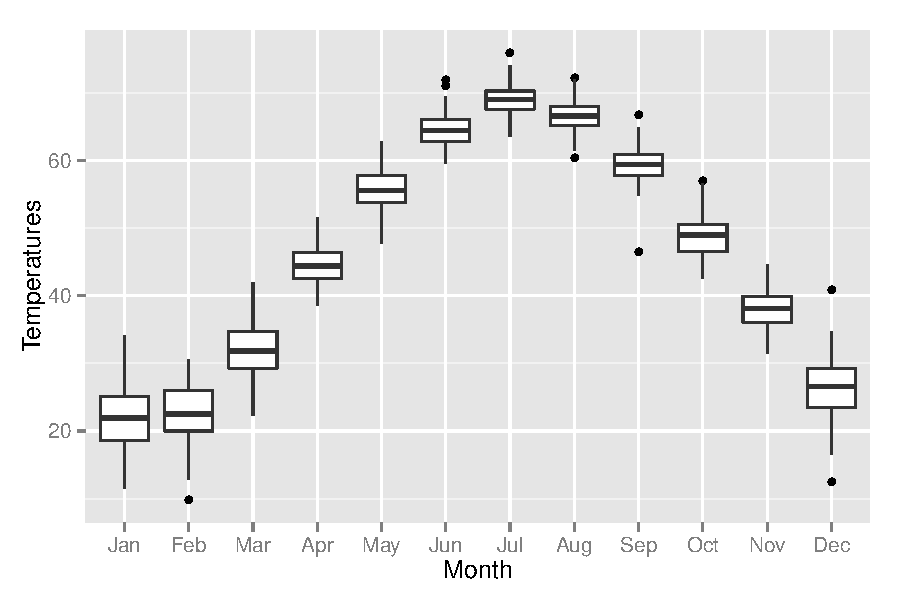
\includegraphics[width=\maxwidth]{figure/graph1_5} 

\end{knitrout}


\caption{This box-and-whiskers plot illustrates the monthly temperatures in degrees Farenheit of Williamstown, Massachusetts as recorded each month from January 1892 to December 2010.}
\end{figure}

\subsection{Analysis}
While the temperature does not fluctuate in the mid-year months (most notably May through September), the winter months (especially January and December) vary greatly in terms of temperature. This is unusual, as one would expect the transitional months of spring and fall to fluctuate the most due to their transient nature.

\section*{Weather 2}
This takes the information from the following link:
\verb+http://web.williams.edu/weather/current_get_date_range.php?start=10_01_2005&end=6_10_2013&interval=24hours+
and creates a data frame of the date compared to the daily temperature
in degrees Farenheit of Williamstown, MA from 2005 to 2013.

\begin{knitrout}
\definecolor{shadecolor}{rgb}{0.969, 0.969, 0.969}\color{fgcolor}\begin{kframe}
\begin{alltt}
x <- \hlfunctioncall{read.table}(\hlstring{"dailyTemp1.txt"})
Date <- x[, 1]
Temperature <- x[, 3]
p <- \hlfunctioncall{ggplot}(x, \hlfunctioncall{aes}(Date, Temperature))
p <- p + \hlfunctioncall{geom_point}(size = 0.6)
\end{alltt}
\end{kframe}
\end{knitrout}


\begin{landscape}
  \begin{figure}
\begin{knitrout}
\definecolor{shadecolor}{rgb}{0.969, 0.969, 0.969}\color{fgcolor}
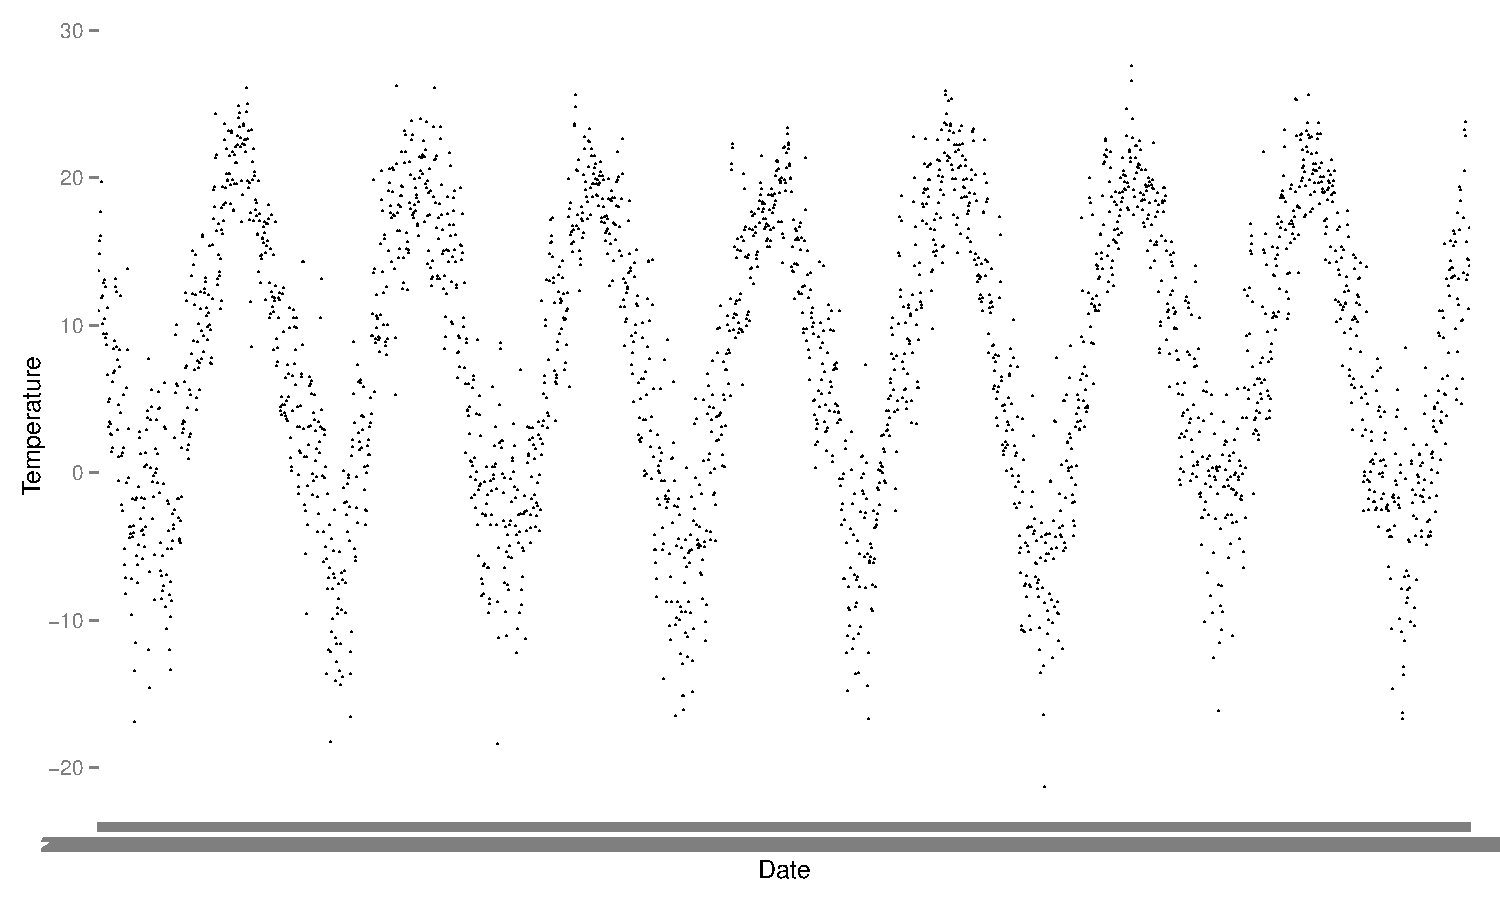
\includegraphics[width=\maxwidth]{figure/graph2Landscape} 

\end{knitrout}


\caption{This scatterplot illustrates the average daily temperatures in degrees Celsius of Williamstown, Massachusetts as recorded from October 1, 2005 to June 10,  2013.}
\end{figure}
\end{landscape}

\subsection{Analysis}
The temperatures fluctuate regularly over the 7 years, reaching a relative minimums of approximately -17 degrees Celsius and relative maximums of approximately 27 degrees Celsius.

\begin{figure}
\begin{knitrout}
\definecolor{shadecolor}{rgb}{0.969, 0.969, 0.969}\color{fgcolor}\begin{kframe}
\begin{alltt}
dateObj <- \hlfunctioncall{as.Date}(Date)
Month <- \hlfunctioncall{month}(dateObj, label = TRUE)
p2 <- \hlfunctioncall{ggplot}(x, \hlfunctioncall{aes}(Month, Temperature))
bp <- p2 + \hlfunctioncall{geom_boxplot}()
bp
\end{alltt}
\end{kframe}
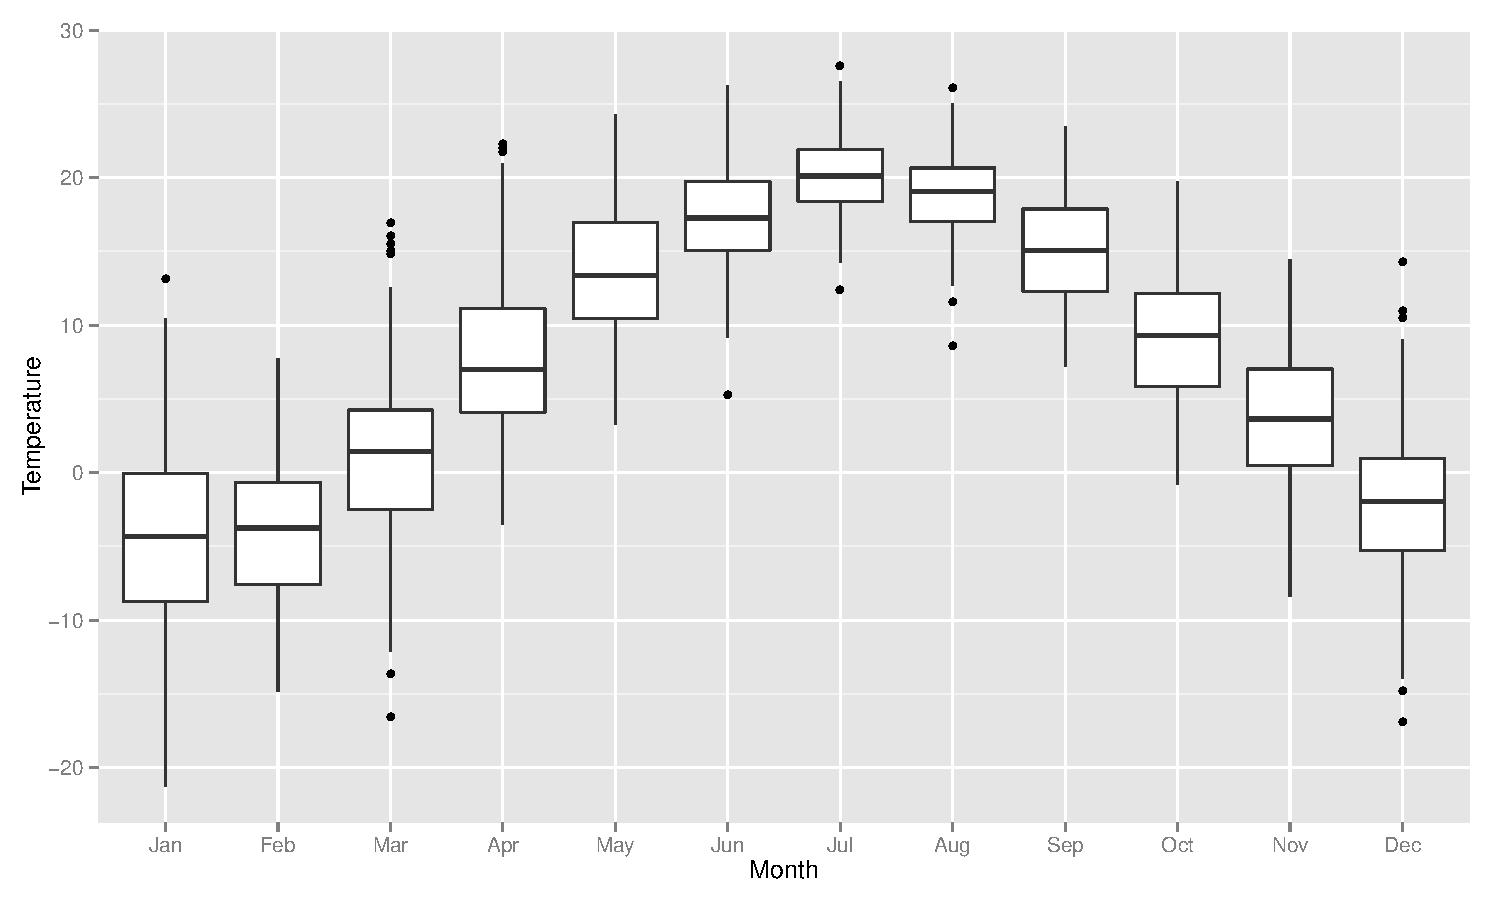
\includegraphics[width=\maxwidth]{figure/graph2BoxPlot} 

\end{knitrout}

\caption{This box-and-whiskers plot illustrates the monthly temperatures in degrees Celsius of Williamstown, Massachusetts as recorded daily from October 1, 2005 to June 10, 2013.
\end{figure}

\subsection{Analysis}
Once again we see that the greatest fluctuation in temperature is found in January and December, while the least fluctuation occurs in June through August.

\section*{Weather 3}
This takes the information from the following link:
 \verb+http://web.williams.edu/weather/archive_get_date_range.php?begin=1_01_1983&end=12_31_2007+
and creates a data frame of the date compared to the daily temperature
in degrees Farenheit of Williamstown, MA from 1983 to 2007.

\begin{knitrout}
\definecolor{shadecolor}{rgb}{0.969, 0.969, 0.969}\color{fgcolor}\begin{kframe}
\begin{alltt}
y <- \hlfunctioncall{read.table}(\hlstring{"dailyTemp2.txt"}, sep = \hlstring{"\textbackslash{}t"})
date <- y[, 1]
y$Temperature <- y[, 2]
dateTrim <- \hlfunctioncall{strtrim}(date, 10)
y$Date <- \hlfunctioncall{as.Date}(dateTrim)
p <- \hlfunctioncall{ggplot}(y, \hlfunctioncall{aes}(Date, Temperature))
p <- p + \hlfunctioncall{geom_point}(size = 0.5, na.rm = TRUE)
p <- p + \hlfunctioncall{layer}(geom = \hlstring{"smooth"}, method = \hlstring{"lm"}, na.rm = TRUE)
\end{alltt}
\end{kframe}
\end{knitrout}


\begin{landscape}
\begin{figure}
\begin{knitrout}
\definecolor{shadecolor}{rgb}{0.969, 0.969, 0.969}\color{fgcolor}
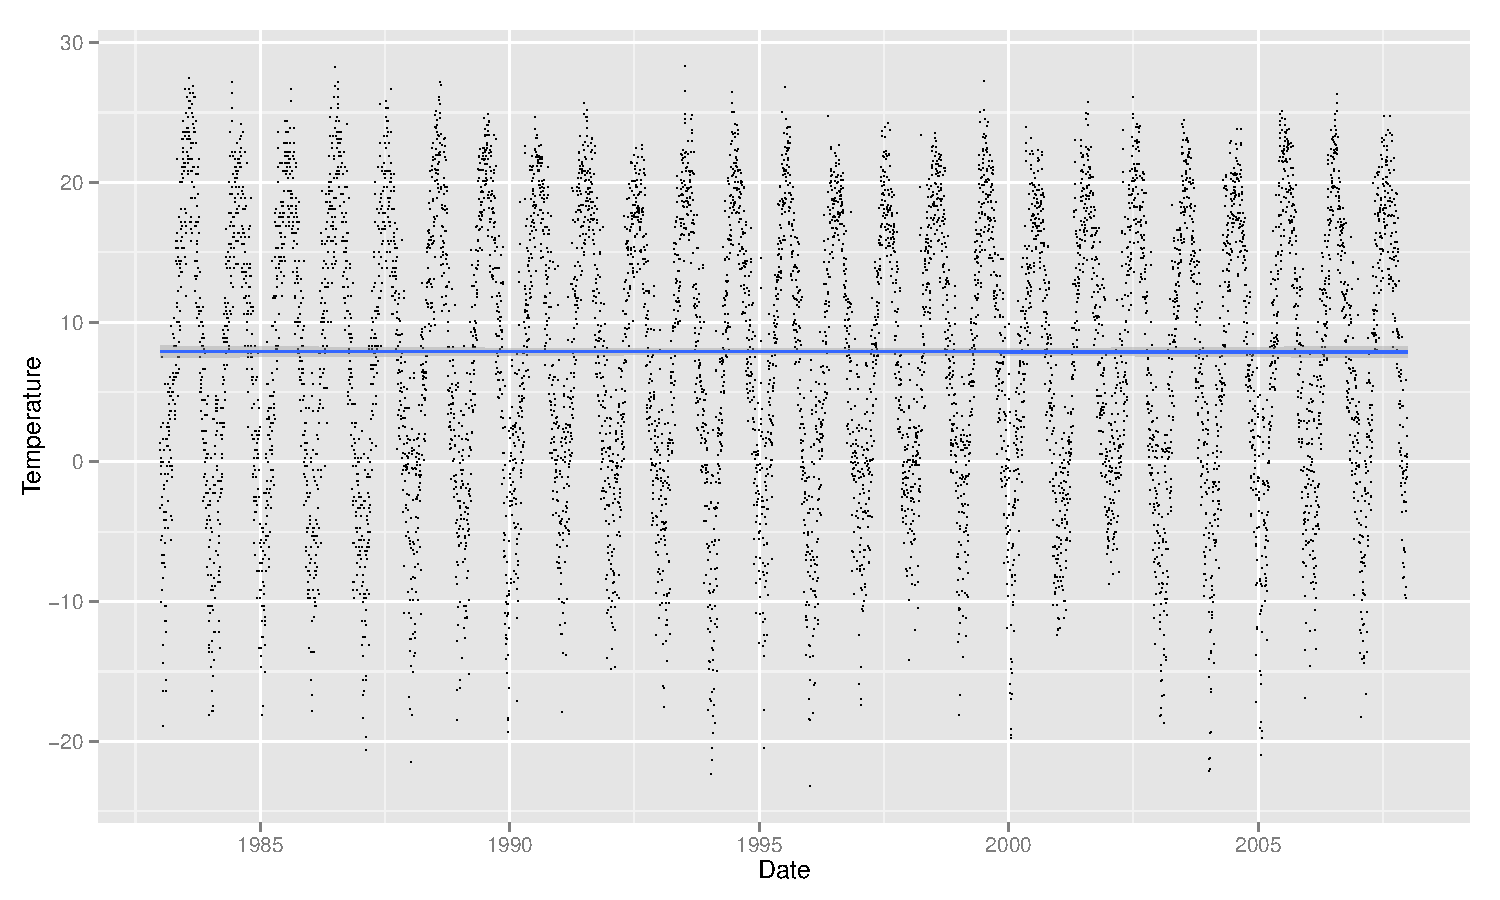
\includegraphics[width=\maxwidth]{figure/graph3Landscape} 

\end{knitrout}


\caption{This scatterplot illustrates the average daily temperatures in
  degrees Celsius of Williamstown, Massachusetts as recorded from
  January 1, 1983 to December 31, 2007.}
\end{figure}
\end{landscape}

\subsection{Analysis}
The temperatures fluctuate regularly over the 24 years, with an average temperature (depicted by the line) of approximately
8 degrees Celsius.

\begin{figure}
\begin{knitrout}
\definecolor{shadecolor}{rgb}{0.969, 0.969, 0.969}\color{fgcolor}\begin{kframe}
\begin{alltt}
dateObj <- \hlfunctioncall{as.Date}(date)
Month <- \hlfunctioncall{month}(dateObj, label = TRUE)
p3 <- \hlfunctioncall{ggplot}(y, \hlfunctioncall{aes}(Month, Temperature))
bp <- p3 + \hlfunctioncall{geom_boxplot}(na.rm = TRUE)
bp
\end{alltt}
\end{kframe}
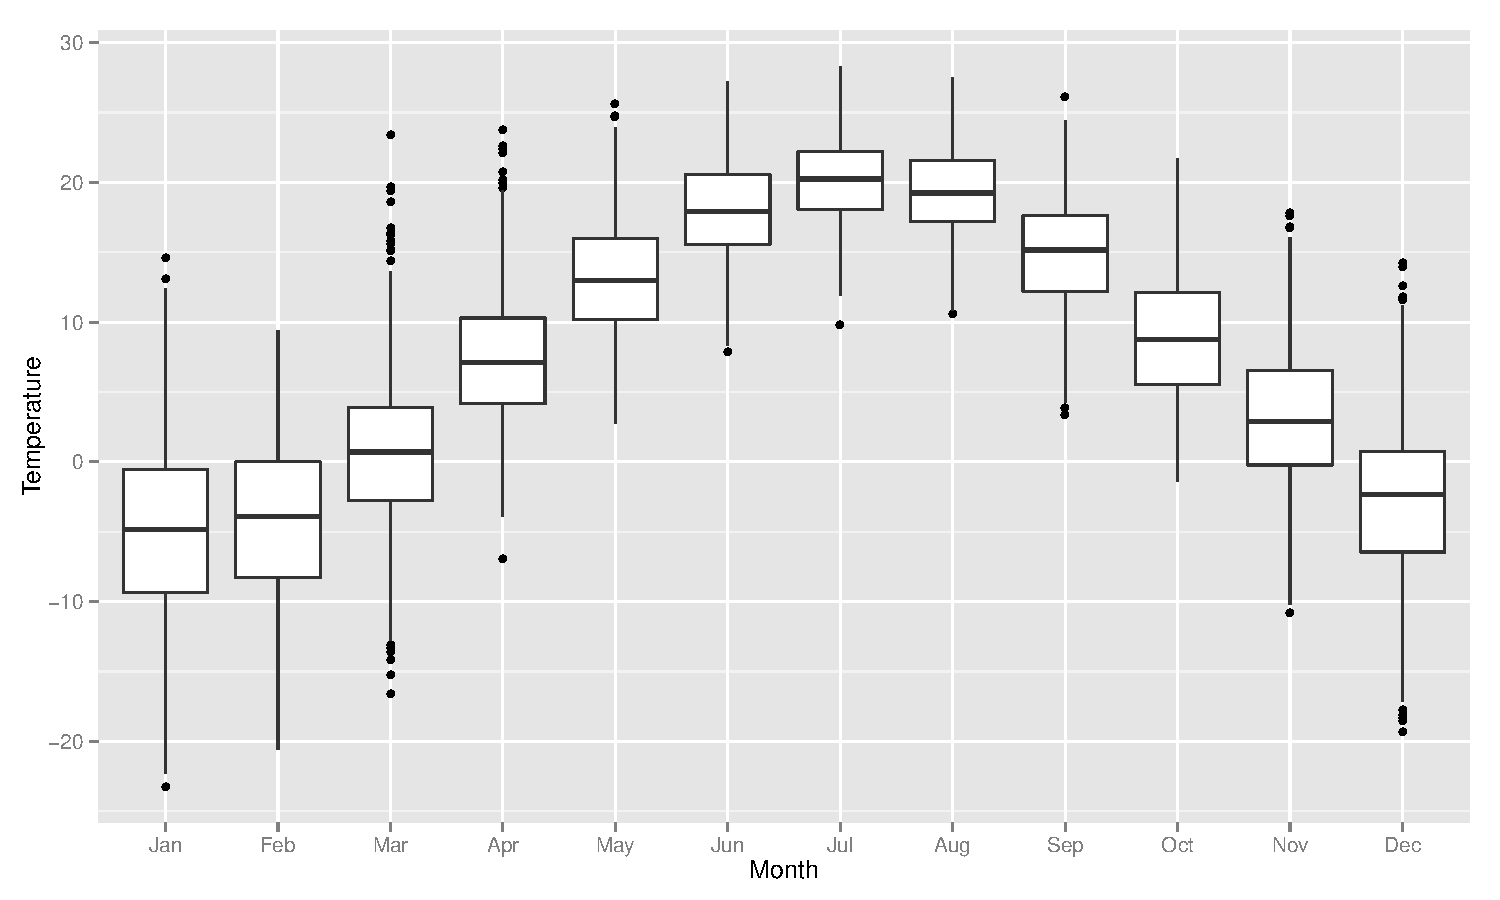
\includegraphics[width=\maxwidth]{figure/graph3BoxPlot} 

\end{knitrout}

\caption{This box-and-whiskers plot illustrates the monthly temperatures in degrees Celsius of Williamstown, Massachusetts as recorded daily from January 1, 1983 to December 31, 2007.}
\end{figure}

\subsection{Analysis}
Again, the monthly temperatures fluctuate the most in the months of January and February but remain more stable in the months of June, July and August.

\end{document}
